\documentclass[10pt,a4paper]{article}
\usepackage{lrec}
\usepackage{multibib,filecontents}
%\newcites{languageresource}{Language Resources}
\usepackage{graphicx}
\usepackage{tabularx}
\usepackage{soul}
\usepackage[ruled]{algorithm2e}
% for eps graphics

\usepackage{tipa}
\let\ipa\textipa
\usepackage{vowel,amssymb}


\usepackage{epstopdf}
%\usepackage[latin1]{inputenc}

\usepackage{fontspec}
\setmainfont{FreeSerif}
%\setmainfont{TeX Gyre Termes}
\usepackage{polyglossia}
\setmainlanguage{english}
\setotherlanguages{sanskrit} %% or other languages
\newfontfamily\devanagarifont[Script=Devanagari]{Annapurna SIL}
\newcommand{\sansk}[1]{\begin{sanskrit}#1\end{sanskrit}}

\usepackage[
pdfauthor={Aalok Sathe},
pdftitle={A Rule-Based System for the Transcription of Sanskrit from the Devanagari Orthography to the International Phonetic Alphabet},
pdfsubject={Linguistics},
pdfkeywords={Transcription, Sanskrit, IPA, Phonetics, WWG algorithm, Devanagari, Computational linguistics},
pdfproducer={XeLaTeX },
pdfcreator={xelatex}]{hyperref}

\usepackage{xstring}

\newcommand{\secref}[1]{\StrSubstitute{\getrefnumber{#1}}{.}{ }}

\title{A Rule-Based System for the Transcription of Sanskrit from the Devanagari Orthography to the International Phonetic Alphabet}

\name{Aalok Sathe}

\address{Department of Math \& Computer Science\\University of Richmond, VA, 23173\\
         \hyperref{mailto:aalok.sathe@richmond.edu}{}{}{aalok.sathe@richmond.edu}\\}


\abstract{
	In this paper, we introduce a system for the transcription of Sanskrit text written using the Devanagari (or Nagari) script-based orthography for Sanskrit, into the International Phonetic Alphabet. We make use of existing literature on closest known approximate pronunciations of sounds as well as prosodic and metric rules for syllabification using the Weerasinghe-Wasala-Gamage algorithm for Sinhala adapted to Sanskrit and the assignment of syllable-weight-determined stress.	
\\
\newline \Keywords{Transcription, Sanskrit, IPA, Phonetics, WWG algorithm, Devanagari, Computational linguistics} }

\begin{document}

\maketitleabstract

\section{Introduction}

The language Sanskrit, being one of the oldest classical languages in existence and having a huge amount of literature, is a topic of frequent study in literature, culture, and linguistics. One hurdle in this process often faced is the lack of a definite and consistent system of phonetic transcription. While the IAST\footnote{International Alphabet of Saskrit Transliteration} and ITRANS\footnote{Indian languages TRANSliteration} have existed and are widely used, they are but alternate means of representation of the same text, not fully capturing the phonological and prosodic features of the text. For new learners or even existing scholars, there exists a steep learning curve as they learn Sanskrit phonology in the context of the language and culture. As such, it would be beneficial to new learners, existing scholars, and unrelated interested parties alike to have at their disposal such a system that would guide their pronunciation as accurately and consistently as possible. It is our personal experience that even after systems such as IAST existing for a while now, students and scholars of Sanskrit worldwide still fumble when it comes to phonology. Other systems have come into being too, however, they either do not solve the problem at hand, or do so inaccurately; examples include the `ICU' system for transliteration of Indic scripts \cite{viswanadha2002transliteration} as well as the website ``Ashtangayoga'' \cite{ashtangayoga}. We propose a system, hence, which we believe will find use as a convenient reference tool as well as a tool for preservation of traditional knowledge by making it available to a wider audience. We detail a system for the transcription of Sanskrit text written using its Devanagari orthography into IPA, complete with the best-known pronunciations of its sounds, rule-based syllabification adapted for Sanskrit from the Weerasinghe-Wasala-Gamage algorithm (hereafter referred to as the ``WWG algorithm'') originally developed for the Sinhala language, and most importantly, stress, a prosodic phonological feature not captured in such existing transcription systems.
In this work, we aim to provide a rule-based algorithmic system, and a computer program based on it, which will provide a consistent transcription given well-formed\footnote{That adhering to the rules of classical Sanskrit phonology and Devanagari orthography} Sanskrit text.


\section{Sanskrit Phonology}

Sanskrit is a classical language with its origins in the Indian subcontinent, and its literature and texts being found in present-day India, Nepal, and neighboring regions.
Sanskrit is one of the official languages of India and shares close common ancestry with most of the modern Indo-Aryan languages spoken in the Indian subcontinent today \cite{emeneau1956india}. It was recorded as the mother-tongue of about 10,000 people in the 2001 census of India \cite{banthia2001census}. While the effective pronunciations of Sanskrit sounds differ from region to region today depending on the speaker's own mother tongue and such linguistic influence, a unified approximation of Sanskrit sounds has been proposed in multiple works. In what follows, we attempt to give a summary of Sanskrit speech sounds.

In Sanskrit, there are multiple singular vowel sounds, as well as diphthongs made by combinations of vowels. The simple vowels are shown in table~3. The diphthongs made through the combination of two vowels, as shown in table~5. All these vowels, whether simple or compound (diphthong), are considered one whole unit in Sanskrit. 
Table~3 also shows the vowel length, which must accordingly be considered during transcription. Diphthongs are long vowels in Sanskrit.
In addition, Sanskrit uses a few other special sounds and treats them as vowels. These are shown in table~4, and are various approximants. For the purposes of transcription, we will consider all these vowels to be a single unit each, with vowel length being the only additional consideration where applicable.

%\begin{figure*}[!ht]
%	\begin{center}
%		%\fbox{\parbox{6cm}{
%		%This is a figure with a caption.}}
%		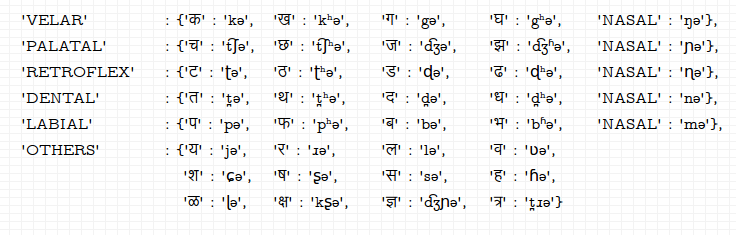
\includegraphics[width=\textwidth]{correspondences.png} 
%		\caption{Sanskrit speech sounds in Devanagari: consonants and non-vowel sounds.}
%	\end{center}
%\end{figure*}

\begin{table*}[ht]
	
	\begin{center}
		\begin{tabular}{|l|c|c|c|c|c|}
			\hline
			 & \textbf{Voiceless }&\textbf{Voiceless aspirated }&\textbf{Voiced }&\textbf{Voiced aspirated }&\textbf{Nasal}\\
			& \textbf{ plosive}&\textbf{ plosive}&\textbf{ plosive}&\textbf{ plosive}&\textbf{}
			\\
			\hline			
			Velar&क : `kə'	&ख : `kʰə'&	ग : `gə'&	घ : `gʰə'& ङ : `ŋə'\\\hline
			Palatal& च : `t͡ɕə'&	छ : `t͡ɕʰə'& ज : `d͡ʑə'&	झ : `d͡ʑʱə'& ञ : `ɲə'\\\hline
			Retroflex& ट : `ʈə'&	ठ : `ʈʰə'& 	ड : `ɖə'& ढ : `ɖʰə'&	ण : `ɳə'\\\hline
			Dental& त : `t̪ə'& 	थ : `t̪ʰə'&	द : `d̪ə'&		ध : `d̪ʰə'& न : `nə'\\\hline
			Labial & प : `pə'& 	फ : `pʰə'& ब : `bə'& 	भ : `bʱə'& म : `mə'\\\hline
			\multicolumn{6}{c}{ }\\\hline
			\multicolumn{6}{|c|}{\textbf{Other sounds}}\\\hline\hline
			Approximants& य : `jə'& 	र : `ɹə'&	ल : `lə'&	व : `ʋə'&\\\hline Fricatives&श : `ɕə'& ष : `ʂə'& 		स : `sə'& 	ह : `ɦə'&\\\hline&
			ळ : `ɭə'&\multicolumn{4}{c|}{ }	%'क्ष' : 'kʂə', 	'ज्ञ' : 'd͡ʒɲə', 	'त्र' : 't̪ɹə'}
			\\\hline
		\end{tabular}
		\caption{Sanskrit speech sounds in Devanagari: consonants and non-vowel sounds.}
	\end{center}
	\label{cons}
\end{table*}


\begin{table*}[ht]
	\begin{center}
		\begin{tabular}{|c|c|c||c|c|c|}
			\hline
			\textbf{Base}&\textbf{Diacritical}&\textbf{IPA}&\textbf{Base} &\textbf{Diacritical}&\textbf{IPA} \\
			\textbf{glyph}& \textbf{combination}&\textbf{symbol}&\textbf{glyph}& \textbf{combination}&{\bf symbol}\\\hline%\hline
			
			\sansk{अ}&&ə& \sansk{आ}& \sansk{ा}&ɑː\\\hline
			\sansk{इ}& \sansk{ि}&i&	\sansk{ई}& \sansk{ी}&iː\\\hline
			\sansk{उ}&\sansk{ ु}&u&
			\sansk{ऊ}& \sansk{ ू}&uː\\\hline
			\sansk{ऋ}&\sansk{ ृ}&ɹ̩&\sansk{ॠ} &\sansk{ ॄ}&ɹ̩ː\\\hline
			\sansk{ऌ}&\sansk{	ॢ}&l̩&\sansk{ॡ} &\sansk{ॣ}&l̩ː\\\hline
			\sansk{ए}&\sansk{ े}&eː& \sansk{ऐ} & \sansk{	ै}&ɑːi\\\hline
			\sansk{ओ}& 	\sansk{ो }&oː&	\sansk{	अाै}&\sansk{ाै}&  ɑːu\\\hline
			\sansk{अं}& \sansk{	ं }&əm&	\sansk{अः}&	\sansk{ः} & əh\\\hline
			\sansk{ॐ} &&oːm&&&%\multicolumn{3}{|c|}{ }
			\\\hline
			
		\end{tabular}
		\caption{Sanskrit speech sounds in Devanagari: vowels and syllabic sounds.}
	\end{center}
	\label{vow}
\end{table*}

%\begin{figure*}[!ht]
%	\begin{center}
%		%\fbox{\parbox{6cm}{
%		%This is a figure with a caption.}}
%		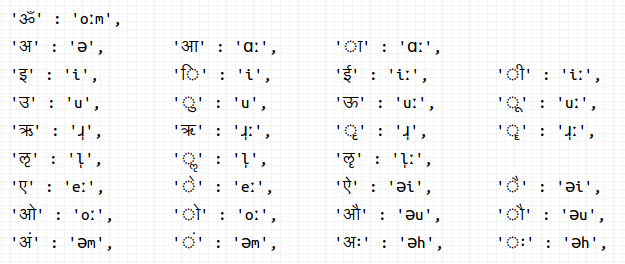
\includegraphics[scale=0.6]{correspondences_vowelsIPA.png} 
%		\caption{Sanskrit speech sounds in Devanagari: vowels and syllabic sounds.}
%	\end{center}
%\end{figure*}



\begin{table*}[ht]
	\begin{center}
		\begin{tabular}{|c|l|l|l|}
			\hline
			&Front&Central&Back\\\hline
			High&\sansk{इ} ([i]), \sansk{ई} ([iː])&&\sansk{उ} ([u]), \sansk{ऊ} ([uː])\\
			Mid&$\phi$,$\hskip0.em\quad\quad$\sansk{ए} ([eː])&\sansk{अ} ([ə]), $\phi$ &$\phi$,$\hskip0.em\quad\quad$ \sansk{ओ} ([oː])\\
			Low&&$\phi$,$\quad\quad$ \sansk{अा} ([ɑː])&\\
			\hline
				
		\end{tabular}\label{vowelsposition}
		\caption{Sanskrit speech sounds in Devanagari: simple vowels. Those toward the left are short versions of the vowel, while those toward the right are long. In case a short or long version of a vowel doesn't exist, a `$\phi$' has been displayed to indicate the lack of it. Blank spaces denote that the vowel is not in the Sanskrit phonemic inventory.}
	\end{center}

\end{table*}


We will base our transcription system upon existing literature on the phonology of Sanskrit \cite{jamison2004sanskrit} as well as a system of correspondences between Devanagari text, IAST, and IPA, in the work `The Original Pronunciation of Sanskrit' \cite{zieba2002original}. We will hence establish a mapping between Sanskrit and IPA symbols \cite{international1999handbook}. As such, table~1 shows the correspondences used for consonants and other non-vowel sounds, while table~2 is the vowel and vowel-like sounds' counterpart.
Sanskrit makes use of special symbols for several compound consonants as well, which we will process not as a whole, but using their constituent components. Fortunately, unicode character combinations for Devanagari define these characters in terms of their constituent components, making it easier for us to process them.
While Sanskrit has many complex phonological processes where sounds interact, a popular one of which is \textit{sandhi}, we need not encode rules of such phonetic interaction except those implied or left ambiguous in the orthography. It is expected of an input phrase to be well-formed, i.e., not having any phonological inconsistencies per the rules of Sanskrit. Given that this program will likely find use in transcription of existing texts, this should not be an issue in most cases. In case an input contains a character that is not present in the Devanagari Sanskrit orthography, the program should notice this, for it will make sure that the input characters are within a pre-specified unicode code-point range.

Another noteworthy consideration is the differential pronunciations of a {\it visarga}, or a `\sansk{ः}'-terminated character. Today, the interpretation of the pronunciation of this sound is slowly shifting towards a new one: sustaining the vowel sound of the previous syllable with an aspirated fricative ([{\it \ipa{h}}]) and duplicating the same vowel after the fricative sound. While this seems to be a rising trend, it did not always use to be so until very recently,  and the sound was supposed to be simply a {[\ipa{h}]}-terminating one, without vowel duplication. As such, we have taken the interpretation of this sound to mean as close as possible to what is believed to have been the pronunciation in the classical Sanskrit era \cite{zieba2002original,jamison2004sanskrit}.

\section{Rule-Based Transcription}

In our program, we will use several one-pass processes to fully transcribe a given text in linear time. In what follows, some of the orthographic intricacies that require us to do so have been described.

\subsection{Shorthand for Nasalization}

The Devanagari Sanskrit orthography has several ways to indicate the presence of a nasal sound, which carries some meaning in the word's semantics. Conventionally, a nasal consonant is only explicitly shown when a phrase ends, or the upcoming character is a Sanskrit vowel\footnote{As detailed in the several tables above. A vowel in the strict phonetic sense is not meant here.}. In the case that the nasal sound is not explicitly shown, an {\it anuswaar} is shown on the character preceding it, and its actual sound is inferred at the time of reading or pronouncing. A nasal can be one of six types, five of which are shown in table~1. The sixth type applies when a sound doesn't fit into any of the five categories among: velar, palatal, retroflex, dental, and labial, which are roughly the descriptions of sounds based on their sites of production. When a sound doesn't fall into any of these categories, for example, a fricative, or a vowel, it shall be called the sixth case, and in this case, the preceding vowel is nasalized, and no additional sound is added. For instance in the word \sansk{संस्कृत} ([sə̃̃s.kɹ̩.t̪ə]) itself, where the {\it anuswar}'s circumstance is not one of the five types mentioned. The specific nasal sound to be used is inferred based on the next sound, if one exists, or is taken to be {[\ipa{m}]}, the bilabial nasal sound, by default.

\subsection{Handling the Default Schwa}

A consonant character in Devanagari Sanskrit, unless explicitly marked {\it halant} (i.e., a schwa-less ``partial'' sound marked using the diacritic \sansk{्}), has an implied schwa with it. For instance, \sansk{ग} may be transcribed as [ɡə], while to yield [ɡ], we would need to mark a lack of schwa as \sansk{ग्}. As such, a removal of schwa may be required when explicitly marking a character {\it halant}, or when combining another vowel after it. In the latter case, it is the way Devanagari is structured in unicode code-points that requires this to be done: when combining a consonant with a non-schwa vowel, one must explicitly remove schwa first, as demonstrated in the following example:
\sansk{गो = ग  +  ो}  $\,$ is the way the character combination takes place in unicode code-points, however, phonologically speaking, it is $\,$
\sansk{गो = ग + ् + ओ} $\,$([ɡoː]), where we are removing the schwa and explicitly adding another vowel, instead of superficially dealing with diacritical marks. When dealing with the phonetic transcription, hence, this needs to be taken care of, since at the surface, it is not apparent what underlying phonological process is taking place.

\begin{table}[]
	
	\begin{center}
		\begin{tabular}{|c|}
			\hline
			\sansk{ऋ} ([ɹ̩]),$\quad$ \sansk{ॠ} ([ɹ̩ː])\\\hline\hline
			\sansk{ऌ} ([l̩]),$\quad$ \sansk{ॡ} ([l̩ː])\\\hline
			
		\end{tabular}
		\caption{Sanskrit speech sounds: special vowels. The first row shows short and long syllabic alveolar approximant sounds, respectively, while similarly, the second row shows short and long lateral approximant ones.}
	\end{center}
	\label{ru}
\end{table}

\begin{table}[]
	
	\begin{center}
		\begin{tabular}{|c|c|c|}
			\hline
			$X$&$X+$\sansk{इ,ए}&$X+$\sansk{उ,अो}\\\hline
			\sansk{अ,अा}&\sansk{ऐ} ([ɑːi])&\sansk{औ} ([ɑːu])\\\hline
			
		\end{tabular}
		\caption{Sanskrit speech sounds: simplified rules of diphthong formation}
	\end{center}
	\label{diphth}
\end{table}

\subsection{Syllabification}

For syllabification, we make use of the WWG algorithm \cite{weerasinghe2005rule} adapted to Sanskrit \cite{gdasa2013sanskritSyllabification}. In the original study, the algorithm was developed to account for the majority of Sinhalese vocabulary which has Sanskrit and Pali origins as well as direct borrowings. As such, the authors note that the algorithm would be similarly applicable to Sanskrit.
As shown in algorithm~\ref{alg1}, we syllabify using groups of vowel-consonant-vowels, of the kind $V_BC_nC_{n-1}\dots C_2C_1V_A$, where $n\geq1$. We apply rules based on the number of such consonants in the central consonant cluster, i.e., $n$. Based on this length and conventional sonority- and meter-based syllabification preferences, we mark the boundaries of the syllables.

\begin{algorithm}[h]
	\label{alg1}
	\SetAlgoLined
	\KwIn{Sanskrit text to be syllabified}
	\texttt{initialize} scope at the beginning of text\;
	\While{end of text not reached}{
		\texttt{move} to next $V_B\mathbb{C}V_A$ group, where $\mathbb{C}$ is a consonant cluster\;
		\uIf{length of cluster $\mathbb{C} = 1$}{
			\texttt{mark} syllable break after $V_B$\;
		}\uElseIf{length of cluster $\mathbb{C} = 2$}{\texttt{mark} syllable break after first $C$ from left\;}\uElseIf{length of cluster $\mathbb{C} = 3$}{
			\uIf{third consonant from left $=$ \sansk{र् or य्} {\bf or} first and second consonants are stops}{\texttt{mark} syllable break after first $C$ from left\;}
			\Else{\texttt{mark} syllable break before first $C$ from right\;}
		}\Else{
			\uIf{first consonant from right $=$ \sansk{र् or य्}}{\texttt{mark} syllable break before second $C$ from right\;}
			\Else{\texttt{mark} syllable break after least sonorous $C$\;}
			}
	}
	\KwResult{Syllabified Sanskrit text\vskip0.5em}
	
\caption{WWG Algorithm adapted to Sanskrit}
\end{algorithm}

\subsubsection{Examples}
%\setmainfont{Doulos SIL}
In what follows, we provide some example Sanskrit words to demonstrate syllabification as carried out using algorithm~\ref{alg1}. For ease of reading, we highlight the consonant cluster in consideration using boldface in the Devanagari text.
\begin{enumerate}
	\item \sansk{कृ\textbf{त}म्} ([kɹ̩.t̪əm]) was split before [t̪] following the rule for a cluster of length one.
	
	\item \sansk{व\textbf{ल्क}लानि} ([ˈʋəl.kə.lɑː.ni]): here, the first two syllables have been demarcated from each other by splitting a consonant cluster of length two.
	
	\item 
	\begin{enumerate}
		\item \sansk{म\textbf{त्स्यः}} ([ˈmət̪.sjəh]): this cluster of length three has been split according to the rule that checks the presence of either \sansk{र्} or \sansk{य्}.
		
		\item
		\sansk{उ\textbf{क्त्वा}} ([ˈuk.t̪ʋɑː]) demonstrates the rule involving two stops, here, \sansk{क् and त्}. As such, we split it after the first stop from the left hand side.
		
		\item
		\sansk{कृ\textbf{त्स्न}म्} ([ˈkɹ̩t̪s.nəm]) is useful to illustrate the `else' condition when the conditions similar to those in 3(a) and 3(b) do not apply.
	\end{enumerate}
	
	\item
	%\begin{enumerate}
		%\item 
		
		\sansk{का\textbf{र्त्स्न्य}म्} ([kɑːɹt̪s.njəm]) contains a \sansk{य्}-terminal cluster of length more than three, and as such, it has been split before the second consonant when scanning from the right hand side.
		
		%\item		
	%\end{enumerate}
	
\end{enumerate}
%\setmainfont{FreeSerif}

\subsection{Assigning Stress}
Once we finish demarcating the syllables, we use traditional prosodic and metric rules to determine the syllables that should receive stress. In Sanskrit, a syllable is either `light' or `heavy' \cite{sridharan2005sanskrit}. A syllable may be considered to be light in the base case, which later acquires the status of being heavy subject to meeting one or more of the following conditions:
\begin{enumerate}
	\item Syllable contains a long vowel or diphthong
	\item Syllable has nasal-terminating vowel sound or nasalized vowel
	\item Syllable is stressed
\end{enumerate}

When a syllable ends into a consonant cluster instead of a single consonant (or none), the syllable receives stress to make it a heavy syllable if it is not already heavy.
For the sake of an example, the syllables of the word \sansk{कुरु{क्षे}त्र} ([ku.ˈɹuk.ʂeː.t̪ɹə]), when taken independently, are of the kind LLHL, with `L' being light and `H' being heavy. However, when considered together, the character \sansk{क्ष्}, which is a compound consonant of \sansk{क् + ष्}, causes the previous non-heavy syllable (-[.ɹuk.]-) to receive stress, and hence become heavy, making the word of the kind LHHL. Interestingly, the third syllable does not receive stress, even though the syllable after it (or on the boundary of the syllable break, i.e., -[.t̪ɹə]) contains a consonant cluster. This is because having the vowel sound \sansk{े} ([eː]) has already caused the third syllable to become heavy.

\vspace{.3\baselineskip}

\section{Software}
Prototype software developed as part of this work may be found at the following link:\\
\hyperref{https://github.com/aalok-sathe/sanskrit_IPA}{}{}{\tt https://github.com/aalok-sathe/sanskrit\_IPA}.


The software, written using Python3, primarily because of inbuilt unicode support, allows the user to transcribe text on the go using a persistent command-prompt design, using a command in the manner: \texttt{transcribe} \textit{text}. The software also has the option to set an input file externally, for large files, and output it in a similarly named file in the same directory. This is especially useful for transcribing large texts.

The software is released under the third version of the GNU General Public License, to support the spirit of free and open-source software, as well as to encourage further development in this regard.

\section{Future Work}
More work along similar lines will be required to truly create a set of tools to represent traditional knowledge in not just Sanskrit, but most of the Indic (of several language families) languages, and eventually, more underrepresented languages of the world. To begin with, systems need to be developed that will ensure backwards transcription compatibility of Devanagari Sanskrit and IPA, as well as those that will be able to transcribe consistently to most of the major ways of representing Sanskrit text today, including ITRANS and IAST.
While developing such a system for Sanskrit is possible using rule-based decision procedures alone for the most part, this may not, and for a fact is not possible for most other modern languages, who rely largely on the speaker's cultural and experiential knowledge of the language for phonetic disambiguation. For such languages as Hindi and Marathi, statistical learning methods will need to be used in addition to rule-based systems to create transcription mechanisms that are as accurate as possible.

\section{Acknowledgments}
We are grateful for helpful comments by and discussion on this and such related topics with Mukund Gokhale, Hema Kshirsagar, Shardul Chiplunkar, and Dieter Gunkel.

The font Annapurna SIL was used to render Devanagari text for the purpose of this manuscript.
This manuscript was typeset using Xe\LaTeX.
% \nocite{*}

\section{Bibliographical References}
\label{main:ref}

\bibliographystyle{lrec}
\bibliography{mybib}


	
%\section{Language Resource References}
%\label{lr:ref}
%\bibliographystylelanguageresource{lrec}
%\bibliographylanguageresource{xample}

\end{document}
